\documentclass[11pt]{article}
\usepackage[margin=1in]{geometry}
\usepackage{amsmath,amssymb,graphicx,booktabs,xcolor,fancyvrb}
\usepackage[colorlinks=true,linkcolor=blue]{hyperref}

\makeatletter
\def\ps@hw{%
  \def\@oddhead{\itshape\small CS 334 HW2 --- Extra Credit\hfill Nathaniel Schrader}%
  \def\@oddfoot{\hfil\small\thepage\hfil}%
  \let\@evenhead\@oddhead \let\@evenfoot\@oddfoot}
\makeatother
\pagestyle{hw}

\fvset{fontsize=\footnotesize,frame=single,numbers=left,numbersep=4pt,xleftmargin=6pt}
\newcommand{\vth}{\vec\theta}
\newcommand{\x}[1]{\vec x^{(#1)}}

\begin{document}
\thispagestyle{hw}

\begin{center}
{\Large\bfseries CS 334 --- Homework 2 Extra Credit}\\[4pt]
{\large Nathaniel Schrader \quad|\quad CS 334 Section 2 \quad|\quad Fall 2026}\\[10pt]
\fbox{\parbox{0.92\textwidth}{\small\centering
\textbf{Honor Code Statement:}\\
THIS HOMEWORK IS MY OWN WORK, WRITTEN WITHOUT COPYING FROM OTHER STUDENTS
OR DIRECTLY FROM LARGE LANGUAGE MODELS SUCH AS CHATGPT.\\
Any collaboration or external resources have been properly acknowledged.\\[4pt]
\textit{Nathaniel Schrader}}}
\end{center}
\vspace{6pt}
\hrule
\vspace{10pt}

\section*{Q4 --- Weighted Linear Regression}

\paragraph{(a)} When some data points are more reliable than others. For example, if some measurements come from a precise instrument and others from a cheap, noisy one, you'd want the precise ones to count more. Another example is weighting recent data more heavily in a time series.

\paragraph{(b)} Let $W$ be the $N\times N$ diagonal matrix with $W_{ii}=w^{(i)}$, and let $\vec r=X\vth-\vec y$, so $r_i=\vth\cdot\x i-y^{(i)}$. Since $W$ is diagonal,
\[
(X\vth-\vec y)^TW(X\vth-\vec y)=\vec r^{\,T}W\vec r=\sum_{i=1}^N w^{(i)}r_i^2=\sum_{i=1}^N w^{(i)}\big(\vth\cdot\x i-y^{(i)}\big)^2,
\]
and $\lambda\|\vth\|_2^2=\lambda\vth^T\vth$. So $J(\vth)=(X\vth-\vec y)^TW(X\vth-\vec y)+\lambda\vth^T\vth$.

\paragraph{(c)} Expanding (using $W=W^T$):
\[
J(\vth)=\vth^TX^TWX\vth-2\vec y^{\,T}WX\vth+\vec y^{\,T}W\vec y+\lambda\vth^T\vth
\]
Take the gradient and set it to zero:
\begin{align*}
\nabla J=2X^TWX\vth-2X^TW\vec y+2\lambda\vth&=0\\
(X^TWX+\lambda I)\vth&=X^TW\vec y\\
\vth^*&=(X^TWX+\lambda I)^{-1}X^TW\vec y
\end{align*}

\paragraph{(d)} From \texttt{linear\_regression.py}:
\VerbatimInput{figures/weighted_ls.py.txt}

\paragraph{(e)} Same sweep as Q3.2(b) but with the weighted fit. Since the fit minimizes weighted error, I measured error with weighted RMS, $\sqrt{\sum_i w^{(i)}r_i^2/\sum_i w^{(i)}}$.
\begin{center}
\begin{minipage}{0.52\textwidth}\centering
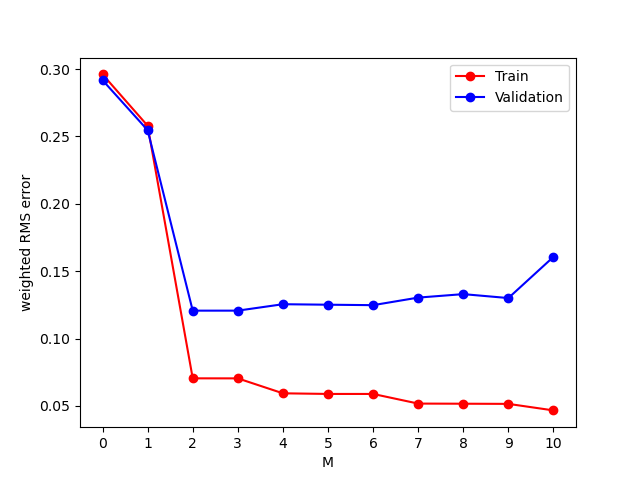
\includegraphics[width=\linewidth]{figures/weighted_rms_vs_M.png}
\end{minipage}\hfill
\begin{minipage}{0.45\textwidth}\centering\small
\begin{tabular}{ccccc}
\toprule
 & \multicolumn{2}{c}{weighted RMS} & \multicolumn{2}{c}{unweighted RMS}\\
$M$ & train & val & train & val\\\midrule
0 & 0.2960 & 0.2917 & 0.465 & 0.421\\
1 & 0.2579 & 0.2547 & 0.529 & 0.472\\
2 & 0.0705 & \textbf{0.1207} & 0.731 & 0.486\\
3 & 0.0704 & 0.1207 & 0.719 & 0.490\\
4 & 0.0594 & 0.1255 & 0.238 & 0.232\\
5 & 0.0589 & 0.1251 & 0.139 & 0.133\\
6 & 0.0589 & 0.1248 & 0.144 & 0.143\\
7 & 0.0517 & 0.1304 & 0.462 & 1.021\\
8 & 0.0516 & 0.1330 & 0.452 & 1.249\\
9 & 0.0515 & 0.1301 & 0.462 & 0.985\\
10 & 0.0467 & 0.1606 & 0.275 & 2.383\\\bottomrule
\end{tabular}
\end{minipage}
\end{center}

\textbf{No, the answer changes to $M=2$} (weighted validation RMS 0.1207, basically tied with $M=3$, so I'd pick the simpler one).

\begin{center}
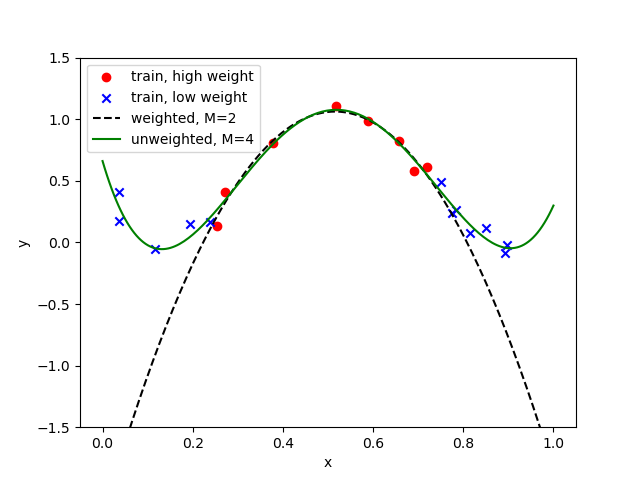
\includegraphics[width=0.55\textwidth]{figures/weighted_fits.png}
\end{center}

The weights are either 1.001 or 0.001, so the fit basically only sees the high-weight points. Those are all in the middle of the curve ($x$ from about 0.25 to 0.72), and a parabola fits that part well. The ends of the curve, which needed $M=4$ before, barely count anymore. Higher degrees just fit noise in the high-weight points. The plot shows this: the weighted $M=2$ fit matches the red points but goes way off at the ends.

\end{document}
